
    \begin{picture} (360.000000,134.592593)(0,0)
    \put(0.0, 0.0){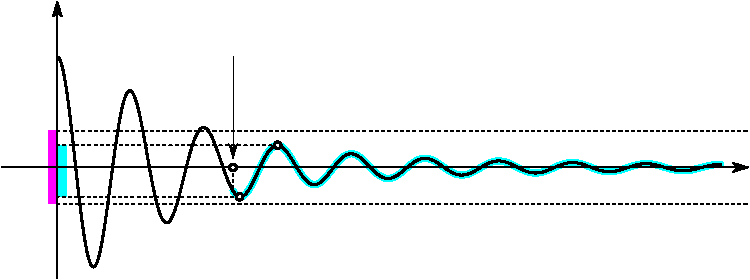
\includegraphics{03ftozeroAok.pdf}}
        \put(111.85, 109.07){\sffamily\itshape \makebox[0pt][c]{$A$}}
    \put(  9.52,  68.54){\sffamily\itshape $+\varepsilon$}
    \put(  9.52,  33.53){\sffamily\itshape $-\varepsilon$}
    \put(186.63, 107.07){\sffamily\itshape \makebox[0pt][l]{%
\parbox{2in}{\centering This $A$ is large enough, because\\
 $f(x)$ is in the right range\\
for all $x\geq A$}}}
\end{picture}
